\documentclass[12pt,a4paper]{article}

\usepackage[left=3cm, right=3cm, top=2cm, bottom = 2cm]{geometry}
\usepackage[utf8]{inputenc}
\usepackage[T1]{fontenc}
\usepackage{lmodern}
\usepackage[UKenglish]{isodate}% http://ctan.org/pkg/isodate

\usepackage{amsmath}
\usepackage{amsfonts}
\usepackage{amssymb}

\usepackage[xindy]{glossaries}
\loadglsentries{acronyms}


\usepackage{tikz}
\usetikzlibrary{automata, positioning, arrows,graphs,matrix,}


\title{Technical Note on Varanus State Transition: Strict or Permissive?}
\author{Matt Luckcuck}

\begin{document}
\maketitle

We can imagine Runtime Verification as being the comparison between two Labelled Transition Systems (LTS), which may have different alphabets, states, and transitions. Hopefully the LTS for the \gls{sua} is similar enough to the LTA for the Specification/Monitor that Runtime Verification is not useless. But, crucially, the LTS for the SUA is hidden from us.

For example, we might have modelled the Specification and produced an LTS:
\begin{center}
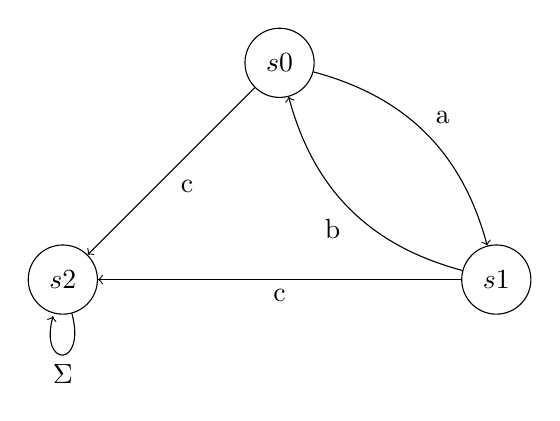
\begin{tikzpicture}[node distance =3cm, auto]
\node[state] (s0) {$s0$};
\node[state] (s1) [below right= of s0] {$s1$};
\node[state] (s2) [below left=of s0] {$s2$};

\path[->] 
		(s0) edge [bend left] node {a} (s1) 
		(s0) edge node {c} (s2) 
		
		(s1) edge [bend left] node {b} (s0) 
		(s1) edge node {c} (s2)
		
		(s2) edge [loop below] node {$\Sigma$} ()  			;

\end{tikzpicture}
\end{center}
\noindent Note: $\Sigma$ represents all CSP events (i.e. every symbol in the Alphabet). Here, the LTS of the Specification ($Spec$) is defined by\\
\begin{center}
$\begin{array}{ll}
States &= \{ s0, s1, s2 \} \\
Alpha &= \{a, b, c\} \\
\end{array} 
$
\\
$Transition = $
\begin{tabular}{l|l|l|l}
$T$  &  $a$ & $b$ & $c$ \\
\hline
$s0$ & $s1$ & $\bot$ & $s2$ \\
$s1$ & $\bot$ & $s0$ & $s2$ \\ 
$s2$ & $s2$ & $s2$ &$s2$ \\
\end{tabular}
\end{center}
Note that here we have two states were a particular transition is not available, represented in the transition table by $\bot$.
 
The LTS for the SUA ($System$) might be an extension of $Spec$: 
\begin{center}
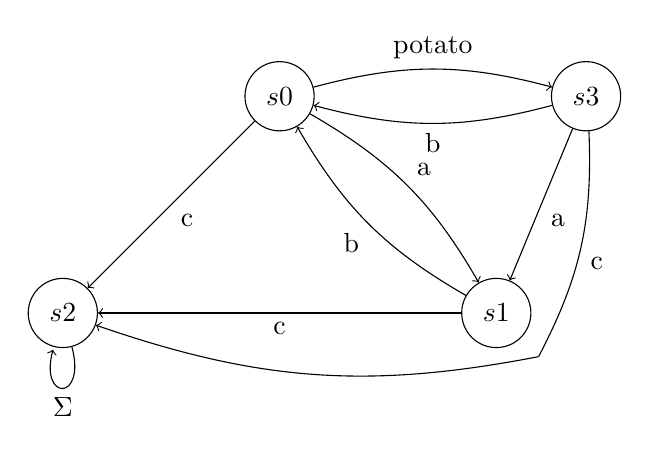
\begin{tikzpicture}[node distance =3cm, auto, bend angle=15]
\node[state] (s0) {$s0$};
\node[state] (s1) [below right= of s0] {$s1$};
\node[state] (s2) [below left=of s0] {$s2$};
\node[state] (s3) [right =of s0] {$s3$};

\node (waypoint) [below right = of s1, xshift = -1.9cm, yshift=1.9cm, minimum width=0mm,inner sep=0mm,outer sep=0mm] {};

\path[->] 
		(s0) edge [bend left] node {a} (s1) 
		(s0) edge node {c} (s2) 
		(s0) edge [bend left] node {potato}  (s3)
		
		(s1) edge [bend left] node {b} (s0) 
		(s1) edge node {c} (s2)
				
		(s2) edge [loop below] node {$\Sigma$} ()  			

		(s3) edge [bend left]  node {b} (s0)
		(s3) edge node {a} (s1)	
		
		(waypoint) edge [bend left] node {} (s2)
		;
\path
(s3) edge [bend left] node {c} (waypoint) ;
\end{tikzpicture}
\end{center}
\noindent The $System$ LTS is defined by\\
\begin{center}
$\begin{array}{ll}
States &= \{ s0, s1, s2, s3 \} \\
Alpha &= \{a, b, c, potato\} \\
\end{array} 
$
\\
$Transition = $
\begin{tabular}{l|l|l|l|l}
$T$  &  $a$ & $b$ & $c$ & $potato$\\
\hline
$s0$ & $s1$ & $\bot$ & $s2$ & $s3$\\
$s1$ & $\bot$ & $s0$ & $s2$ & $\bot$\\ 
$s2$ & $s2$ & $s2$ &$s2$ & $s2$\\
$s3$ & $s1$ & $s0$ & $s3$ & $\bot$
\end{tabular}
\end{center}

The two LTSs above are different, the $System$ LTS has an extra state and another symbol in its alphabet. Crucially, though, we don't know \textit{why} they are different.
Maybe:
\begin{itemize}
\item the system is doing something wrong, $Spec$ should included $potato$ and it was mistakenly not included in the specification;, or,
\item the specification that $Spec$ is based on didn't include $potato$ and it doesn't need to know about it because system safety doesn't depend on the $potato$ event.
\end{itemize}
So \Varanus provides two modes, permissive and strict, to deal with these two possibilities.  Strict mode handles situation 1, above; if \Varanus hears $potato$ then it would see this as an error. 
Permissive mode handles situation 2: if \Varanus hears $potato$ then it would remain in the current state.

Using RV usually assumes that we do not have a formal representation of the SUA, hence we do not have the $System$ LTS described above. However, we might see some events in the alphabet of the SUA $Alpha(System)$ if it produces them at runtime. If an event produced by the SUA is not in the alphabet of the specification ($Alpha(Spec)$) then we have no mapping in the transition function for it \textit{and} we don't know why (for the reasons mentioned above). 
But we do know that if an event is in $Alpha(Spec)$ but not available in a given state, then if the SUA produces that event it must be an error. 
This produces the transition function:
\begin{center}
\begin{tabular}{l|l|l|l|l}
$T$  &  $a$ & $b$ & $c$ & $potato$\\
\hline
$s0$ & $s1$ & $E$ & $s2$ & $\bot$\\
$s1$ & $E$ & $s0$ & $s2$ & $\bot$\\ 
$s2$ & $s2$ & $s2$ &$s2$ & $\bot$\\
\end{tabular}
\end{center}
\noindent Where $E$ represents an error, and if we hear $potato$ in any state then we have no information. These are the situations where the mode (strict or permissive) decided the outcome.

In general terms, the two modes work as follows.
In \textit{strict} mode, if an event from the \gls{sua} is not in the alphabet of the monitor, then \Varanus aborts; here, the model states exactly what the system should do. However, in \textit{permissive} mode, if an event from the \gls{sua} is not in the monitor's alphabet, then \Varanus ignores it and stays in the current state; here, the model is an abstract specification of what the system should do. Remember: even in permissive mode, if the \gls{sua} performs an event that is in the monitor's alphabet but not available in the current state, \Varanus will conclude that it is a failing trace.
The transition tables below show the outcome in each mode:\\
~\\
\begin{minipage}{0.45\textwidth}
\begin{center}
\textbf{Strict mode}
\begin{tabular}{l|l|l|l|l}
$T$  &  $a$ & $b$ & $c$ & $potato$\\
\hline
$s0$ & $s1$ & $E$ & $s2$ & $E$\\
$s1$ & $E$ & $s0$ & $s2$ & $E$\\ 
$s2$ & $s2$ & $s2$ &$s2$ & $E$\\
\end{tabular}
\end{center}
\end{minipage}
\noindent \begin{minipage}{0.45\textwidth}
\begin{center}
\textbf{Permissive mode}
\begin{tabular}{l|l|l|l|l}
$T$  &  $a$ & $b$ & $c$ & $potato$\\
\hline
$s0$ & $s1$ & $E$ & $s2$ & $s0$\\
$s1$ & $E$ & $s0$ & $s2$ & $s1$\\ 
$s2$ & $s2$ & $s2$ &$s2$ & $s2$\\
\end{tabular}
\end{center}
\end{minipage} \\
\noindent In strict mode, all the transitions for the $potato$ event become errors because we do not have a mapping for them in the transition function and therefore the \gls{sua} must be misbehaving. 
Conversely, in permissive mode all the transitions for the $potato$ event become recursions, because we assume that the $poato$ event is one we should ignore and await one of the `important' events in our alphabet.

If $next(s, a)$ is the state transition function that maps the current state($s$) and an event in the alphabet ($a$) to the next state in machine $M$, and $Alpha(M)$ gives the alphabet of $M$ then we can define a state transition function for each mode as follows:\\

\begin{center}
\textbf{Strict mode}
\[
 next_{strict}(s, a) =
  \begin{cases} 
   E & \text{if } a \notin Alpha(M) \\
   next(s,a) & \text{otherwise } 
  \end{cases}
\]
\end{center}

\begin{center}
\textbf{Permissive mode}
\[
 next_{permissive}(s, a) =
  \begin{cases} 
   s & \text{if } a \notin Alpha(M) \\
   next(s,a) & \text{otherwise } 
  \end{cases}
\]
\end{center}
\noindent (Again, $E$ represents an error.)

\end{document}